%% chapter5_slides.tex
%% Chapter 5: Fejer Monotonicity and Fixed Point Iterations
%% Bauschke & Combettes --- Convex Analysis and Monotone Operator Theory in
%% Hilbert Spaces, 2nd ed. (CMS Books in Mathematics, Springer, 2017)
%% Compile: pdflatex -interaction=nonstopmode chapter5_slides.tex  (run twice)

\documentclass[aspectratio=169,10pt]{beamer}

\usetheme{Madrid}
\usecolortheme{seahorse}
\usefonttheme{professionalfonts}
\setbeamertemplate{footline}[frame number]
\setbeamertemplate{navigation symbols}{}

%% Packages
\usepackage{amsmath,amssymb,mathtools}
\usepackage{graphicx}
\usepackage{listings}
\usepackage{xcolor}
\usepackage{booktabs}
\usepackage{microtype}

\graphicspath{{figures/}}

%% Python listings style
\lstdefinestyle{python}{
  language=Python,
  basicstyle=\ttfamily\scriptsize,
  keywordstyle=\color{blue!80!black}\bfseries,
  commentstyle=\color{green!50!black}\itshape,
  stringstyle=\color{orange!80!black},
  numbers=left,
  numberstyle=\tiny\color{gray},
  stepnumber=1,
  numbersep=4pt,
  frame=single,
  backgroundcolor=\color{gray!7},
  breaklines=true,
  showstringspaces=false,
  tabsize=4,
  captionpos=b,
}

%% Maths shortcuts
\newcommand{\cH}{\mathcal{H}}
\newcommand{\Fix}{\operatorname{Fix}}
\newcommand{\R}{\mathbb{R}}
\newcommand{\N}{\mathbb{N}}
\newcommand{\norm}[1]{\left\|#1\right\|}
\newcommand{\inner}[2]{\left\langle #1 \mid #2 \right\rangle}
\newcommand{\weakto}{\rightharpoonup}
\newcommand{\dC}{d_C}
\newcommand{\Id}{\operatorname{Id}}
\newcommand{\conv}{\operatorname{conv}}

%% Title info
\title[Convex Analysis \& MOT -- Ch.5]{Convex Analysis and Monotone Operator Theory in Hilbert Spaces}
\subtitle{Chapter 5: Fej\'er Monotonicity and Fixed Point Iterations}
\author{Based on Bauschke \& Combettes}
\institute{CMS Books in Mathematics, Springer, 2nd ed., 2017}
\date{}

% ---------------------------------------------------------------
\begin{document}
% ---------------------------------------------------------------

\begin{frame}
  \titlepage
\end{frame}

\begin{frame}{Chapter Outline}
  \tableofcontents
\end{frame}

% =================================================================
\section{Notation and Recap}
% =================================================================

\begin{frame}[allowframebreaks]{Notation You'll Need}

  \textbf{Ambient space.} $\cH$ is a real Hilbert space with inner
  product $\inner{\cdot}{\cdot}$ and norm $\norm{\cdot}$. All sequences
  $(x_n)_{n\in\N}$ live in $\cH$ unless stated otherwise.

  \begin{itemize}
    \item $C$: a nonempty subset of $\cH$ --- the ``target set'' a
      sequence is measured against (often $C=\Fix T$).
    \item $B(x;\rho)=\{y\in\cH:\norm{y-x}\le\rho\}$: closed ball.
    \item $\dC(x)=\inf_{y\in C}\norm{x-y}$: \textbf{distance function}
      to $C$ (how far $x$ is from the nearest point of $C$).
    \item $P_C$: the \textbf{metric projector} onto a closed convex $C$,
      $P_Cx=\operatorname*{argmin}_{y\in C}\norm{x-y}$ (recap from Ch.~4);
      $P_C$ is firmly nonexpansive and $\Fix P_C=C$.
    \item $\Fix T=\{x\in D: Tx=x\}$: fixed point set of $T:D\to D$.
    \item $x_n\weakto x$: \textbf{weak} convergence
      ($\inner{x_n}{z}\to\inner{x}{z}$ for every $z\in\cH$);
      $x_n\to x$: \textbf{strong} (norm) convergence
      ($\norm{x_n-x}\to0$). Strong $\Rightarrow$ weak, not conversely in
      infinite dimensions.
    \item A \textbf{weak sequential cluster point} of $(x_n)$ is any $x$
      such that $x_{k_n}\weakto x$ for some subsequence $(x_{k_n})$.

  \framebreak

    \item \textbf{Nonexpansive}: $\norm{Tx-Ty}\le\norm{x-y}$;
      \textbf{firmly nonexpansive}: a stronger $1/2$-averaged property
      (Ch.~4); \textbf{$\alpha$-averaged} ($\alpha\in\,]0,1[\,$):
      $T=(1-\alpha)\Id+\alpha R$ for some nonexpansive $R$.
    \item \textbf{Asymptotic regularity} of a Picard-type sequence:
      $x_n-Tx_n\to0$.
    \item \textbf{Demiclosedness principle} (Cor.~4.28): if $T$ is
      nonexpansive, $x_{k_n}\weakto x$, and $Tx_{k_n}-x_{k_n}\to0$, then
      $x\in\Fix T$. \emph{This is the standard bridge from ``the
      residual vanishes'' to ``the cluster point is a fixed point.''}
    \item $\ell^1_+(\N)$: nonnegative real sequences $(\xi_n)$ with
      $\sum_{n\in\N}\xi_n<+\infty$ (\textbf{summable} sequences).
    \item $\conv S$, $\overline{\conv}\,S$: convex hull / closed convex
      hull of $S\subset\cH$.

  \framebreak

    \item \textbf{From Ch.~4 (recap).} A nonexpansive $T$ need not send
      the naive (Banach--Picard) iteration $x_{n+1}=Tx_n$ to a fixed
      point --- e.g.\ $T=-\Id$ on $\cH\ne\{0\}$ cycles $x_0,-x_0,x_0,\dots$
      forever. Averaging (relaxing) the step is the fix; this chapter
      supplies the abstract machinery (\emph{Fej\'er monotonicity})
      that powers essentially every convergence proof for such
      relaxed/iterative schemes.
    \item \textbf{Roadmap of the chapter.} \S5.1 isolates the single
      structural property --- ``never move farther from any point of
      $C$'' --- and proves everything that follows from it alone (weak
      convergence, shadow-sequence strong convergence, linear rates).
      \S5.2--5.3 show that KM iterations and compositions of averaged
      operators automatically produce Fej\'er monotone sequences, so
      \S5.1's toolbox applies directly. \S5.4 relaxes the definition to
      allow summable slack (\emph{quasi}-Fej\'er), covering perturbed /
      inexact iterations. \S5.5 builds \emph{ergodic} (Ces\`aro-averaged)
      convergence results on top of the same machinery, for sequences
      that themselves need not converge.
  \end{itemize}
\end{frame}

% =================================================================
\section{5.1 Fej\'er Monotone Sequences}
% =================================================================

\begin{frame}{5.1 The Idea, in Plain Language}
  \textbf{Fej\'er monotonicity, informally:} a sequence $(x_n)$ is
  Fej\'er monotone with respect to a set $C$ if it \emph{never gets
  farther away from any point of $C$} as $n$ increases. It is a very
  weak notion --- it says nothing about \emph{where} $(x_n)$ is going,
  only that its distance to each fixed target point $x\in C$ is
  non-increasing.

  \vspace{1em}
  \textbf{Why this is useful.} It is exactly the property that dozens
  of fixed-point / projection / splitting algorithms produce ``for
  free'' from a one-line convexity computation, yet it is already
  strong enough to force: boundedness, convergence of $\norm{x_n-x}$
  for every $x\in C$, and (with one more mild hypothesis) full weak
  convergence of $(x_n)$ itself. It is the single load-bearing concept
  behind the convergence theory of Chapters 4--5.
\end{frame}

\begin{frame}{5.1 Definition and First Example}
  \begin{block}{Definition 5.1 (Fej\'er monotonicity)}
    Let $C$ be a nonempty subset of $\cH$ and let $(x_n)_{n\in\N}$ be a
    sequence in $\cH$. Then $(x_n)_{n\in\N}$ is \textbf{Fej\'er
    monotone with respect to $C$} if
    $$(\forall x\in C)(\forall n\in\N)\quad \norm{x_{n+1}-x}\le\norm{x_n-x}. \tag{5.1}$$
    \emph{Symbols:} $x$ ranges over the \emph{whole} target set $C$
    (not just one point); the inequality must hold \emph{simultaneously}
    for every $x\in C$ and every step $n$.
  \end{block}

  \begin{block}{Example 5.3 (Picard iterates of a nonexpansive map)}
    Let $D$ be nonempty closed convex, $T:D\to D$ nonexpansive with
    $\Fix T\ne\emptyset$, $x_0\in D$, and $x_{n+1}=Tx_n$. Then $(x_n)$
    is Fej\'er monotone with respect to $\Fix T$: for $p\in\Fix T$,
    $\norm{x_{n+1}-p}=\norm{Tx_n-Tp}\le\norm{x_n-p}$.
  \end{block}
  This one-line computation is the seed from which \emph{every}
  convergence result in this chapter grows.
\end{frame}

\begin{frame}[allowframebreaks]{5.1 Proposition 5.4: The Basic Toolbox}
  \begin{block}{Proposition 5.4}
    Let $C\subset\cH$ be nonempty and $(x_n)$ Fej\'er monotone w.r.t.\ $C$.
    Then:
    \begin{enumerate}
      \item[(i)] $(x_n)$ is \textbf{bounded}.
      \item[(ii)] For every $x\in C$, $(\norm{x_n-x})_{n\in\N}$
        \textbf{converges}.
      \item[(iii)] $(\dC(x_n))_{n\in\N}$ is \textbf{decreasing} and
        converges.
      \item[(iv)] For every $m,n\in\N$: $\norm{x_{n+m}-x_n}\le2\dC(x_n)$.
    \end{enumerate}
  \end{block}

  \textbf{Proof.}
  \begin{itemize}
    \item[(i)] Fix $x\in C$. By (5.1), $\norm{x_n-x}\le\norm{x_0-x}$
      for all $n$, so $(x_n)$ lies in $B(x;\norm{x_0-x})$: bounded.
    \item[(ii)] Immediate from (5.1): a nonincreasing sequence of
      nonnegative reals converges.
    \item[(iii)] Taking the infimum over $x\in C$ in (5.1) gives
      $\dC(x_{n+1})\le \dC(x_n)$ for all $n$; nonincreasing and bounded
      below by $0$, hence convergent.

  \framebreak

    \item[(iv)] Let $x\in C$. Triangle inequality plus (5.1) applied
      $m$ times:
      $$\norm{x_{n+m}-x_n}\le\norm{x_{n+m}-x}+\norm{x_n-x}\le2\norm{x_n-x}.$$
      Taking the infimum over $x\in C$ gives the claim. $\blacksquare$
  \end{itemize}

  \textbf{Reading it.} (ii) is the key structural fact: Fej\'er
  monotonicity gives you, \emph{for free}, that the whole family of
  scalar sequences $\{\norm{x_n-x}\}_{x\in C}$ converges --- not just
  one of them. This ``simultaneous convergence for every target point''
  is exactly the raw material an Opial-type argument needs to pin down
  a \emph{single} weak limit (next slide).
\end{frame}

\begin{frame}[allowframebreaks]{5.1 Step-by-Step: The Core Weak Convergence Theorem}
  \begin{block}{Theorem 5.5}
    Let $C$ be a nonempty subset of $\cH$ and $(x_n)$ Fej\'er monotone
    w.r.t.\ $C$. Suppose that \textbf{every weak sequential cluster
    point} of $(x_n)$ belongs to $C$. Then $(x_n)$ converges weakly to
    a point in $C$.
  \end{block}

  \textbf{Why this is the ``core'' theorem of the chapter.} Every weak
  convergence result later (KM iteration, compositions of averaged
  operators, POCS, ...) is an application of \emph{exactly} this
  statement, after checking its one hypothesis (cluster points lie in
  $C$) via the demiclosedness principle. We now prove it from scratch,
  combining Proposition 5.4(ii) with an Opial-type uniqueness argument
  (the same mechanism reused for Theorem 5.36 in \S5.5).

  \textbf{Step 1 (boundedness $\Rightarrow$ cluster points exist).} By
  Proposition 5.4(i), $(x_n)$ is bounded. Every bounded sequence in a
  Hilbert space has at least one weak sequential cluster point (weak
  compactness of bounded sets). By hypothesis, every such cluster point
  lies in $C$.

  \framebreak

  \textbf{Step 2 (a polarization identity).} Let $x,z\in C$ be
  \emph{any} two points of $C$. Expanding the square,
  $$(\forall n\in\N)\quad 2\inner{x_n}{x-z}=\norm{x_n-z}^2-\norm{x_n-x}^2+\norm{x}^2-\norm{z}^2. \tag{$\ast$}$$
  By Proposition 5.4(ii), both $\norm{x_n-z}$ and $\norm{x_n-x}$
  converge as $n\to\infty$ (since $x,z\in C$). Hence the right-hand
  side of $(\ast)$ converges, so
  $$\inner{x_n}{x-z}\to\ell\quad\text{for some }\ell\in\R.$$

  \textbf{Step 3 (two cluster points must agree).} Suppose $x$ and $z$
  are \emph{both} weak sequential cluster points of $(x_n)$ that lie in
  $C$ (by Step 1, such points exist and belong to $C$): say
  $x_{k_n}\weakto x$ and $x_{l_n}\weakto z$ along subsequences. Taking
  the limit of $\inner{x_{k_n}}{x-z}$ along the first subsequence gives
  $\inner{x}{x-z}=\ell$; taking the limit of $\inner{x_{l_n}}{x-z}$
  along the second gives $\inner{z}{x-z}=\ell$. Subtracting,
  $$\norm{x-z}^2=\inner{x}{x-z}-\inner{z}{x-z}=\ell-\ell=0,$$
  so $x=z$.

  \framebreak

  \textbf{Step 4 (unique cluster point $\Rightarrow$ weak convergence).}
  Steps 1--3 show that $(x_n)$ is bounded and has \emph{exactly one}
  weak sequential cluster point, call it $x^\ast\in C$. A standard fact
  about bounded sequences in a Hilbert space (weak topology on bounded
  sets is metrizable / sequential-compactness argument): if every
  subsequence of a bounded sequence has a further subsequence
  converging weakly to the \emph{same} point $x^\ast$, then the whole
  sequence converges weakly to $x^\ast$. Hence
  $$x_n\weakto x^\ast\in C. \qquad\blacksquare$$

  \textbf{Takeaway.} Fej\'er monotonicity supplies Step 2's convergence
  of $\norm{x_n-x}$ ``for free''; the only external ingredient needed
  in any application is verifying that weak cluster points land in
  $C$ --- almost always done via the demiclosedness principle.
\end{frame}

\begin{frame}{5.1 Weak Need Not Be Strong: Example 5.6}
  \begin{block}{Example 5.6}
    Suppose $\cH$ is infinite-dimensional and let $(x_n)$ be an
    \textbf{orthonormal sequence} in $\cH$. Then $(x_n)$ is Fej\'er
    monotone with respect to $\{0\}$ (indeed $\norm{x_{n+1}-0}=1=\norm{x_n-0}$
    for all $n$), and $x_n\weakto0$, but $x_n\not\to0$ (since
    $\norm{x_n-0}=1\not\to0$).
  \end{block}
  \textbf{Lesson.} Theorem 5.5 genuinely only gives \emph{weak}
  convergence in general --- strong convergence of a Fej\'er monotone
  sequence with respect to a closed convex set needs an extra
  ingredient, which is exactly what Propositions 5.7, 5.10 and
  Theorems 5.11--5.12 supply next.
\end{frame}

\begin{frame}[allowframebreaks]{5.1 The Shadow Sequence Always Converges Strongly}
  \begin{block}{Proposition 5.7}
    Let $C$ be nonempty closed convex and $(x_n)$ Fej\'er monotone
    w.r.t.\ $C$. Then the \textbf{shadow sequence} $(P_Cx_n)_{n\in\N}$
    converges \textbf{strongly} to a point $z\in C$, and
    $$(\forall x\in C)\quad \lim\norm{x_n-z}^2\le\norm{x-z}^2+\lim\norm{x_n-x}^2. \tag{cf.\ 5.2--5.3}$$
  \end{block}

  \textbf{Intuition.} Even when $(x_n)$ itself only converges weakly
  (Example 5.6), its \emph{projections onto $C$} are forced into a
  genuine Cauchy sequence, because $\dC(x_n)$ is decreasing (Prop.\
  5.4(iii)) and this decrease exactly controls how far $P_Cx_n$ can
  move between two indices.

  \textbf{Proof sketch.} Expanding via the three-point identity for
  projections (Ch.~3) and simplifying with (5.1) yields, for all
  $m,n\in\N$,
  $$\norm{P_Cx_n-P_Cx_{n+m}}^2\le \dC^2(x_n)-\dC^2(x_{n+m}). \tag{5.2}$$
  Since $(\dC(x_n))_n$ converges (Prop.\ 5.4(iii)), the right side
  $\to0$ as $m,n\to\infty$: $(P_Cx_n)$ is Cauchy in the \emph{complete}
  set $C$, hence converges strongly to some $z\in C$. The stated
  inequality then follows from Corollary 3.16 (an expansion of
  $\norm{x_n-x}^2$ split through $P_Cx_n$) and letting $n\to\infty$.
  $\blacksquare$

  \begin{block}{Corollary 5.8}
    If in addition $x_n\weakto x$ with $x\in C$, then $P_Cx_n\to x$.
  \end{block}
  \emph{I.e.}, once you know the weak limit lies in $C$, the shadow
  sequence's strong limit must coincide with it.
\end{frame}

\begin{frame}{5.1 Affine Subspaces: A Free Upgrade}
  \begin{block}{Proposition 5.9}
    Let $C$ be a \textbf{closed affine subspace} of $\cH$ and $(x_n)$
    Fej\'er monotone w.r.t.\ $C$. Then:
    \begin{enumerate}
      \item[(i)] $P_Cx_n=P_Cx_0$ for every $n$ (the shadow sequence is
        \emph{constant} from the start!).
      \item[(ii)] If every weak sequential cluster point of $(x_n)$
        belongs to $C$, then $x_n\weakto P_Cx_0$.
    \end{enumerate}
  \end{block}
  \textbf{Why affine subspaces are special.} The proof exploits that
  $y_\alpha:=\alpha P_Cx_0+(1-\alpha)P_Cx_n\in C$ for \emph{every}
  $\alpha\in\R$ (not just $\alpha\in[0,1]$, since $C$ is affine, not
  merely convex); letting $\alpha\to+\infty$ in a Fej\'er-type
  inequality forces $P_Cx_n=P_Cx_0$ exactly. This is the mechanism
  behind the von Neumann--Halperin theorem in \S5.3.
\end{frame}

\begin{frame}[allowframebreaks]{5.1 Strong Convergence: Raik's Theorem and Linear Rates}
  \begin{block}{Proposition 5.10 (Raik)}
    Let $C\subset\cH$ with $\operatorname{int}C\ne\emptyset$ and $(x_n)$
    Fej\'er monotone w.r.t.\ $C$. Then $(x_n)$ converges
    \textbf{strongly} in $\cH$ and $\sum_{n\in\N}\norm{x_{n+1}-x_n}<+\infty$.
  \end{block}
  \textbf{Idea.} Pick $x\in\operatorname{int}C$ with a ball
  $B(x;\rho)\subset C$; project the segment $[x_n,x_{n+1}]$ radially
  from $x$ to build auxiliary points $z_n\in B(x;\rho)\subset C$, apply
  (5.1) to $z_n$, and expand to get
  $$\norm{x_{n+1}-x}^2\le\norm{x_n-x}^2-2\rho\norm{x_{n+1}-x_n}.$$
  Summing over $n$ telescopes the left side and bounds
  $\sum_n\norm{x_{n+1}-x_n}\le\norm{x_0-x}^2/(2\rho)<\infty$: a
  \emph{summable} increment sequence forces the Cauchy property.

  \framebreak

  \begin{block}{Theorem 5.11}
    Let $C$ be nonempty closed convex and $(x_n)$ Fej\'er monotone
    w.r.t.\ $C$. TFAE: (i) $(x_n)\to$ a point of $C$ strongly;
    (ii) $(x_n)$ has a strong cluster point in $C$;
    (iii) $\underline{\lim}\,\dC(x_n)=0$.
  \end{block}
  \emph{Reading it:} for Fej\'er monotone sequences w.r.t.\ a closed
  convex $C$, strong convergence is \textbf{equivalent} to the much
  weaker-looking condition that the distance to $C$ merely has a
  vanishing subsequence --- because $\dC(x_n)$ is already monotone
  (Prop.\ 5.4(iii)), $\liminf=0$ upgrades automatically to a genuine
  limit $0$, and then Prop.\ 5.7 finishes the job.

  \begin{block}{Theorem 5.12 (linear convergence)}
    If in addition $\dC(x_{n+1})\le\kappa\,\dC(x_n)$ for some
    $\kappa\in[0,1[\,$ and all $n$, then $(x_n)\to x\in C$ with the
    \textbf{explicit rate}
    $$(\forall n\in\N)\quad \norm{x_n-x}\le2\kappa^n\dC(x_0). \tag{5.8}$$
  \end{block}
  \emph{Proof idea:} Theorem 5.11 gives strong convergence to some
  $x\in C$; then Prop.\ 5.4(iv), $\norm{x_n-x_{n+m}}\le2\dC(x_n)$,
  combined with the geometric bound $\dC(x_n)\le\kappa^n\dC(x_0)$ and
  letting $m\to\infty$, gives (5.8) directly.
\end{frame}

\begin{frame}{5.1 Iterating Firmly Quasinonexpansive Families}
  \begin{block}{Proposition 5.13}
    Let $(T_n)_{n\in\N}$ be firmly quasinonexpansive operators with
    $C=\bigcap_{n\in\N}\Fix T_n\ne\emptyset$, $(\lambda_n)\subset\,]0,2[\,$,
    $x_0\in\cH$, and $x_{n+1}=x_n+\lambda_n(T_nx_n-x_n)$. Then $(x_n)$
    is \textbf{Fej\'er monotone} w.r.t.\ $C$, and:
    $$\textstyle\sum_{n\in\N}\lambda_n(2-\lambda_n)\norm{T_nx_n-x_n}^2\le \dC^2(x_0),$$
    with weak convergence to a point of $C$ once cluster points lie in
    $C$, and strong convergence when $\operatorname{int}C\ne\emptyset$
    or $\underline\lim\dC(x_n)=0$.
  \end{block}
  This is a \emph{single} statement that already covers a moving
  family of operators $T_n$ (not just one fixed $T$) --- a foretaste of
  the flexibility that \S5.2--5.3's constant-operator theorems will
  exploit.
\end{frame}

\begin{frame}[fragile]{Python: \S5.1 --- Fej\'er Monotonicity in Action}
  \begin{lstlisting}[style=python]
import numpy as np

def T(x):
    """Metric projection onto the closed unit disk in R^2."""
    n = np.linalg.norm(x)
    return x / n if n > 1 else x

x = np.array([3.0, 4.0])          # x0
target_set_pt = np.array([0.6, 0.8])   # one point x in C = Fix(T)
dists = [np.linalg.norm(x - target_set_pt)]
for _ in range(10):
    x = T(x)                       # Picard iteration (Example 5.3)
    dists.append(np.linalg.norm(x - target_set_pt))

print("distances ||x_n - x||:", np.round(dists, 4))
# -> [4.0, 0.0, 0.0, 0.0, ...]  monotone NON-INCREASING (5.1) --
# here it even reaches 0 after one step, since T maps radially onto
# the boundary and x0 is already a positive multiple of (0.6, 0.8).
  \end{lstlisting}
  \textbf{Note.} With plain Picard steps ($\lambda\equiv1$) the disk
  projection example converges in a single step; \S5.2 uses relaxed
  steps ($\lambda=0.5$) precisely so that convergence is gradual and we
  can watch Fej\'er monotonicity unfold over several iterations.
\end{frame}

\begin{frame}{Figure: A Fej\'er Monotone Sequence of Distances}
  \centering
  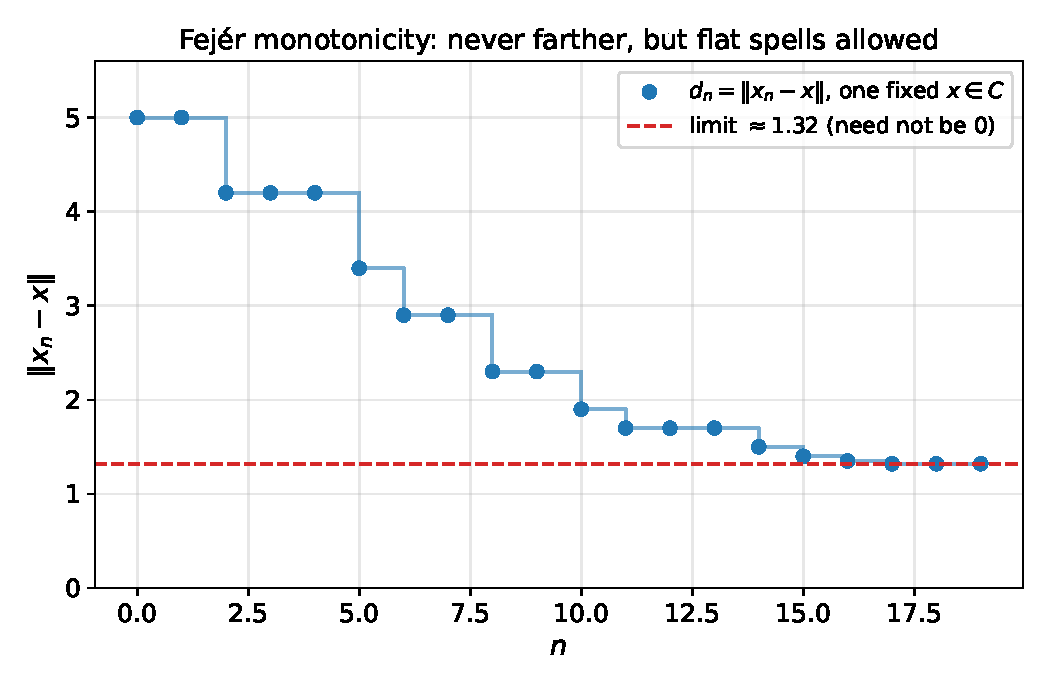
\includegraphics[width=0.72\linewidth]{fejer_monotone_distances.pdf}\\
  {\scriptsize $d_n=\norm{x_n-x}$ for one fixed $x\in C$: the sequence
  never increases, but flat stretches (equal consecutive values) are
  perfectly allowed --- Fej\'er monotonicity is a \emph{non-strict}
  monotonicity condition, and the limit need not be $0$ (Example 5.6).}
\end{frame}

% =================================================================
\section{5.2 Krasnosel'ski\u{i}--Mann Iteration}
% =================================================================

\begin{frame}{5.2 Running Example (Used Throughout This Section)}
  Let $\cH=\R^2$, $C=$ closed unit disk, and
  $$T(x)=\begin{cases}x/\norm{x}, & \norm{x}>1,\\ x, & \norm{x}\le1,\end{cases}$$
  the metric projection onto $C$ (firmly nonexpansive, $\Fix T=C$).
  Start at $x_0=(3,4)$, $\norm{x_0}=5$; since $x_0=5\cdot(0.6,0.8)$
  lies on the ray through the boundary point $(0.6,0.8)$, every
  iterate below stays on that ray, and writing $x_n=r_n\,(0.6,0.8)$ the
  KM recursion collapses to the scalar recursion
  $$r_{n+1}=(1-\lambda)r_n+\lambda,\qquad r_0=5,\ \lambda=0.5,$$
  reproducing
  $$r_0=5,\ r_1=3,\ r_2=2,\ r_3=1.5,\ r_4=1.25,\ r_5=1.125,\dots\to1,$$
  i.e.\ $x_n\to x^\ast=(0.6,0.8)\in\Fix T$. We verify Fej\'er
  monotonicity of this exact sequence w.r.t.\ $\Fix T=C$ below.
\end{frame}

\begin{frame}[allowframebreaks]{5.2 Theorem 5.14: Asymptotic Regularity Suffices}
  \begin{block}{Theorem 5.14}
    Let $D$ be nonempty closed convex, $T:D\to D$ nonexpansive,
    $\Fix T\ne\emptyset$, $x_0\in D$, $x_{n+1}=Tx_n$ (\textbf{plain
    Picard}), and suppose $x_n-Tx_n\to0$ (\textbf{asymptotic
    regularity}). Then:
    \begin{enumerate}
      \item[(i)] $(x_n)\weakto$ a point in $\Fix T$.
      \item[(ii)] If $D=-D$ and $T$ is \textbf{odd}
        ($T(-x)=-Tx$), then $(x_n)\to$ a point in $\Fix T$
        \textbf{strongly}.
    \end{enumerate}
  \end{block}

  \textbf{Proof of (i).} By Example 5.3, $(x_n)$ is Fej\'er monotone
  w.r.t.\ $\Fix T$. Let $x$ be a weak sequential cluster point, say
  $x_{k_n}\weakto x$. Since $Tx_{k_n}-x_{k_n}\to0$ (asymptotic
  regularity), the demiclosedness principle (Cor.\ 4.28) gives
  $x\in\Fix T$. Theorem 5.5 finishes the proof. $\blacksquare$

  \framebreak

  \textbf{Why asymptotic regularity is the crux.} Theorem 5.14 assumes
  $x_n-Tx_n\to0$ as a \emph{hypothesis} --- plain Picard iteration of a
  nonexpansive $T$ does \textbf{not} guarantee this automatically (a
  rotation is nonexpansive, has a fixed point, yet $x_n-Tx_n$ does not
  shrink to $0$: the orbit just cycles). This is exactly the gap that
  the Krasnosel'ski\u{i}--Mann relaxation is designed to close:
  averaging with $\Id$ \emph{forces} asymptotic regularity as a
  \emph{consequence} of the algorithm, rather than needing it as an
  extra assumption.
\end{frame}

\begin{frame}[allowframebreaks]{5.2 Step-by-Step: Groetsch's KM Convergence Theorem}
  \begin{block}{Theorem 5.15 (Groetsch)}
    Let $D$ be nonempty closed convex, $T:D\to D$ nonexpansive with
    $\Fix T\ne\emptyset$, $(\lambda_n)_{n\in\N}\subset[0,1]$ with
    $\sum_{n\in\N}\lambda_n(1-\lambda_n)=+\infty$, and $x_0\in D$. Set
    $$(\forall n\in\N)\quad x_{n+1}=x_n+\lambda_n(Tx_n-x_n). \tag{5.15}$$
    Then: (i) $(x_n)$ is Fej\'er monotone w.r.t.\ $\Fix T$;
    (ii) $(Tx_n-x_n)\to0$ strongly; (iii) $(x_n)\weakto$ a point in
    $\Fix T$.
  \end{block}

  \textbf{Step 1 (expand the square).} Fix $y\in\Fix T$. Using the
  Hilbert-space identity
  $\norm{(1-\lambda)a+\lambda b}^2=(1-\lambda)\norm a^2+\lambda\norm b^2
  -\lambda(1-\lambda)\norm{a-b}^2$ with $a=x_n-y$, $b=Tx_n-y$,
  $\lambda=\lambda_n$:
  $$\norm{x_{n+1}-y}^2=(1-\lambda_n)\norm{x_n-y}^2+\lambda_n\norm{Tx_n-y}^2-\lambda_n(1-\lambda_n)\norm{Tx_n-x_n}^2.$$

  \textbf{Step 2 (nonexpansiveness kills the middle term).} Since
  $Ty=y$, $\norm{Tx_n-y}=\norm{Tx_n-Ty}\le\norm{x_n-y}$, so
  $$\norm{x_{n+1}-y}^2\le\norm{x_n-y}^2-\lambda_n(1-\lambda_n)\norm{Tx_n-x_n}^2. \tag{5.16}$$
  This already proves \textbf{(i)}: $\norm{x_{n+1}-y}\le\norm{x_n-y}$
  for every $y\in\Fix T$, i.e.\ (5.1) holds with $C=\Fix T$.

  \framebreak

  \textbf{Step 3 (telescope and sum).} Summing (5.16) for
  $n=0,\dots,N-1$ telescopes:
  $$\textstyle\sum_{n=0}^{N-1}\lambda_n(1-\lambda_n)\norm{Tx_n-x_n}^2\le\norm{x_0-y}^2-\norm{x_N-y}^2\le\norm{x_0-y}^2.$$
  Letting $N\to\infty$, the bound is uniform, so
  $$\textstyle\sum_{n\in\N}\lambda_n(1-\lambda_n)\norm{Tx_n-x_n}^2\le\norm{x_0-y}^2<+\infty.$$
  Since $\sum_n\lambda_n(1-\lambda_n)=+\infty$ by hypothesis, this
  forces $\underline\lim_n\norm{Tx_n-x_n}=0$.

  \textbf{Step 4 ($\norm{Tx_n-x_n}$ is itself non-increasing).}
  Directly from (5.15) and nonexpansiveness,
  $$\norm{Tx_{n+1}-x_{n+1}}\le\norm{Tx_{n+1}-Tx_n}+(1-\lambda_n)\norm{Tx_n-x_n}
  \le\norm{x_{n+1}-x_n}+(1-\lambda_n)\norm{Tx_n-x_n}=\norm{Tx_n-x_n}. \tag{5.17}$$

  \framebreak

  \textbf{Step 5 (upgrade liminf to a genuine limit --- proves (ii)).}
  A monotone non-increasing sequence with a subsequence tending to $0$
  must itself converge to $0$. Combining Steps 3--4:
  $$\lim_{n\to\infty}\norm{Tx_n-x_n}=0. \qquad\text{(proves (ii))}$$

  \textbf{Step 6 (cluster points are fixed points --- proves (iii)).}
  By Step 2, $(x_n)$ is Fej\'er monotone w.r.t.\ $\Fix T$, hence bounded
  (Prop.\ 5.4(i)) and possesses weak sequential cluster points. If
  $x_{k_n}\weakto x$, then $Tx_{k_n}-x_{k_n}\to0$ (Step 5) and the
  demiclosedness principle (Cor.\ 4.28) gives $x\in\Fix T$. Theorem 5.5
  now gives $x_n\weakto$ a (single) point of $\Fix T$. $\blacksquare$

  \textbf{Takeaway.} The whole proof is: (5.1)-type inequality
  $\Rightarrow$ Fej\'er monotone $\Rightarrow$ bounded, plus a
  telescoping-sum argument $\Rightarrow$ residual $\to0$
  $\Rightarrow$ demiclosedness $\Rightarrow$ cluster points in
  $\Fix T$ $\Rightarrow$ Theorem 5.5 closes the loop. This is
  \emph{exactly} the Theorem 5.5 machinery from \S5.1, applied to the
  concrete operator $x\mapsto x+\lambda(Tx-x)$.
\end{frame}

\begin{frame}{5.2 Running Example: Verifying Fej\'er Monotonicity Numerically}
  With $\lambda\equiv0.5$, $x_0=(3,4)$, $\Fix T=C$ (the whole disk),
  target point $x^\ast=(0.6,0.8)\in\Fix T$:
  \begin{center}
  \begin{tabular}{c c c c}
    \toprule
    $n$ & $x_n$ & $r_n=\norm{x_n}$ & $\norm{x_n-x^\ast}$ \\
    \midrule
    0 & $(3.000,4.000)$ & $5.000$ & $4.000$ \\
    1 & $(1.800,2.400)$ & $3.000$ & $2.000$ \\
    2 & $(1.200,1.600)$ & $2.000$ & $1.000$ \\
    3 & $(0.900,1.200)$ & $1.500$ & $0.500$ \\
    4 & $(0.750,1.000)$ & $1.250$ & $0.250$ \\
    5 & $(0.675,0.900)$ & $1.125$ & $0.125$ \\
    \bottomrule
  \end{tabular}
  \end{center}
  Both columns $r_n$ and $\norm{x_n-x^\ast}$ are \textbf{strictly
  decreasing} here (a stronger property than Fej\'er monotonicity
  requires, which only forbids \emph{increase}) -- consistent with
  (5.16): equality $\norm{x_{n+1}-y}=\norm{x_n-y}$ would require
  $Tx_n=x_n$, i.e.\ $x_n$ already a fixed point, which never happens
  here for $n<\infty$. In fact $\norm{x_n-x^\ast}=4\cdot0.5^n\to0$:
  \textbf{geometric} decay, since $e_n:=r_n-1$ satisfies
  $e_{n+1}=(1-\lambda)e_n=0.5\,e_n$.
\end{frame}

\begin{frame}{Figure: The Running Example, Visualized}
  \centering
  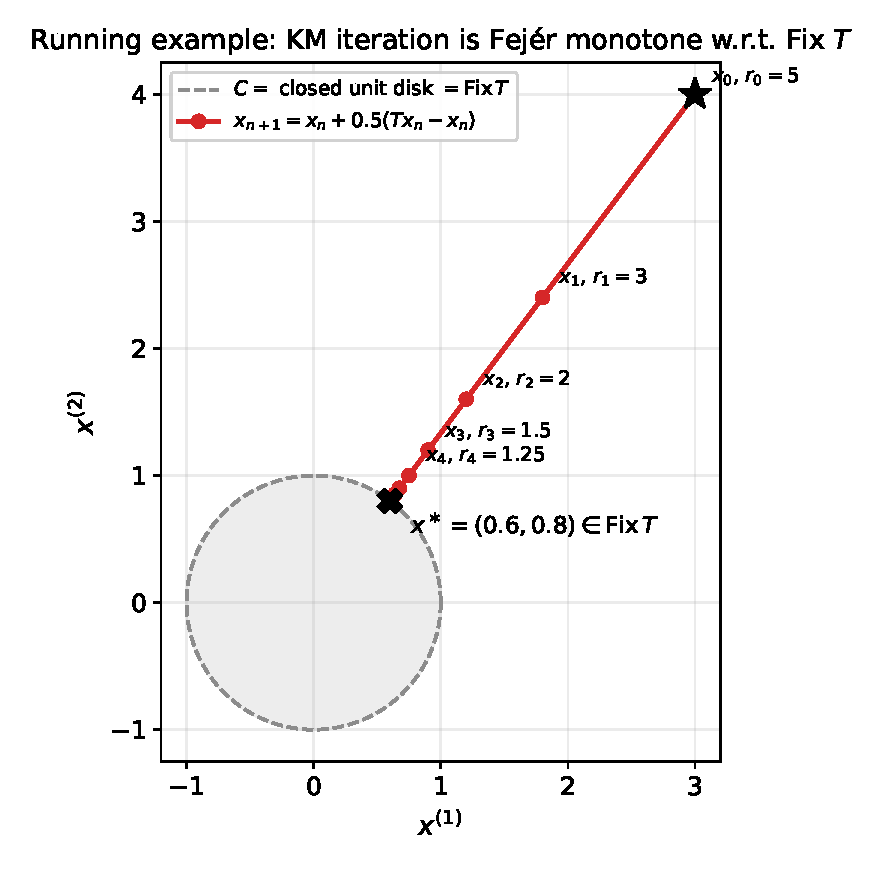
\includegraphics[width=0.62\linewidth]{km_disk_trajectory.pdf}\\
  {\scriptsize KM iteration $x_{n+1}=x_n+0.5(Tx_n-x_n)$ for the
  disk-projection example: the iterates spiral inward along a fixed
  ray toward $x^\ast=(0.6,0.8)\in\Fix T$, always getting no farther
  from any point of $\Fix T=C$ (the shaded disk).}
\end{frame}

\begin{frame}[allowframebreaks]{5.2 Averaged Operators and Firmly Nonexpansive Operators}
  \begin{block}{Proposition 5.16}
    Let $\alpha\in\,]0,1[\,$, $T:\cH\to\cH$ be $\alpha$-averaged with
    $\Fix T\ne\emptyset$, $(\lambda_n)\subset[0,1/\alpha]$ with
    $\sum_n\lambda_n(1-\alpha\lambda_n)=+\infty$, $x_0\in\cH$, and
    $x_{n+1}=x_n+\lambda_n(Tx_n-x_n)$. Then (i) $(x_n)$ is Fej\'er
    monotone w.r.t.\ $\Fix T$; (ii) $Tx_n-x_n\to0$ strongly; (iii)
    $x_n\weakto$ a point in $\Fix T$.
  \end{block}
  \textbf{Proof idea.} Set $R=(1-1/\alpha)\Id+(1/\alpha)T$
  (nonexpansive by Prop.\ 4.35, same $\Fix$) and $\mu_n=\alpha\lambda_n$;
  then the recursion rewrites as $x_{n+1}=x_n+\mu_n(Rx_n-x_n)$ with
  $(\mu_n)\subset[0,1]$, $\sum\mu_n(1-\mu_n)=\infty$ --- \emph{exactly}
  Theorem 5.15 applied to $R$ instead of $T$. \emph{So Groetsch's
  theorem for nonexpansive $T$ already contains the averaged-operator
  case, via this change of operator.}

  \begin{block}{Corollary 5.17}
    $T$ \textbf{firmly nonexpansive} ($=\tfrac12$-averaged),
    $(\lambda_n)\subset[0,2]$ with $\sum_n\lambda_n(2-\lambda_n)=\infty$:
    same conclusions (i)--(iii). \emph{Proof:} apply Prop.\ 5.16 with
    $\alpha=1/2$.
  \end{block}

  \framebreak

  \begin{block}{Example 5.18}
    $T$ firmly nonexpansive, $\Fix T\ne\emptyset$, plain Picard
    $x_{n+1}=Tx_n$ (i.e.\ $\lambda_n\equiv1$ in Cor.\ 5.17, which
    trivially satisfies $\sum2(1)=\infty$): $(x_n)\weakto$ a point in
    $\Fix T$ --- \emph{no relaxation is even needed} when $T$ is
    already firmly nonexpansive.
  \end{block}

  \begin{block}{Corollary 5.19 (compositions and combinations)}
    For a \emph{finite family} $(T_i)_{i\in I}$ of averaged operators
    with $\bigcap_i\Fix T_i\ne\emptyset$, a relaxed KM-type update built
    from a convex combination of finite \emph{compositions}
    $T_{i(k,1)}\cdots T_{i(k,m_k)}$ (with weights $\omega_k$ summing to
    $1$, and an averagedness constant $\alpha$ computed explicitly from
    the $\alpha_i$'s and the composition/combination structure) again
    converges weakly to a point of $\bigcap_i\Fix T_i$.
  \end{block}
  \emph{This single corollary already unifies compositions, convex
  combinations, and relaxation of averaged operators into one weakly
  convergent scheme --- the abstract engine behind \S5.3's POCS-type
  algorithms.}
\end{frame}

\begin{frame}[allowframebreaks]{5.2 Two Concrete Feasibility Algorithms}
  \begin{block}{Example 5.21 (String-averaged relaxed projections)}
    $(C_i)_{i\in I}$ closed convex, $C=\bigcap_iC_i\ne\emptyset$,
    $T_i=(1-\beta_i)\Id+\beta_iP_{C_i}$, $\beta_i\in\,]0,2[\,$; set
    $x_{n+1}=\sum_{k=1}^p\omega_kT_{i(k,1)}\cdots T_{i(k,m_k)}x_n$.
    Then $x_n\weakto$ a point of $C$. \emph{(Corollary 5.19 with
    $\lambda_n\equiv1$, $\alpha_i=\beta_i/2$.)}
  \end{block}

  \begin{block}{Example 5.22 (Parallel projection algorithm)}
    $(C_i)_{i\in I}$ closed convex, $C=\bigcap_iC_i\ne\emptyset$,
    $(\omega_i)_{i\in I}$ positive with $\sum_i\omega_i=1$,
    $(\lambda_n)\subset[0,2]$ with $\sum_n\lambda_n(2-\lambda_n)=\infty$;
    set
    $$x_{n+1}=x_n+\lambda_n\Bigl(\textstyle\sum_{i\in I}\omega_iP_ix_n-x_n\Bigr). \tag{5.22}$$
    Then $x_n\weakto$ a point of $C$. \emph{Proof:} $T=\sum_i\omega_iP_i$
    is a convex combination of firmly nonexpansive maps, hence firmly
    nonexpansive (Ex.\ 4.7) with $\Fix T=\bigcap_i\Fix P_i=C$; apply
    Cor.\ 5.17.
  \end{block}
  \textbf{Contrast with \S5.3.} Here \emph{all} sets $C_i$ are
  consulted \emph{simultaneously} at every step (parallel); \S5.3's
  POCS algorithm instead consults them \emph{one at a time in sequence}
  (composition) --- both are instances of the same general machinery
  (Cor.\ 5.19 vs.\ Theorem 5.23).
\end{frame}

\begin{frame}[fragile]{Python: \S5.2 --- The KM Iteration on the Running Example}
  \begin{lstlisting}[style=python]
import numpy as np

def T(x):
    """Metric projection onto closed unit disk (firmly nonexpansive)."""
    n = np.linalg.norm(x)
    return x / n if n > 1 else x.copy()

def km_iteration(x0, lam, n_steps):
    """x_{n+1} = x_n + lam*(T(x_n) - x_n), constant relaxation lam."""
    x = np.array(x0, dtype=float)
    hist = [x.copy()]
    for _ in range(n_steps):
        x = x + lam * (T(x) - x)
        hist.append(x.copy())
    return np.array(hist)

xstar = np.array([0.6, 0.8])
orbit = km_iteration([3.0, 4.0], lam=0.5, n_steps=8)
r = np.linalg.norm(orbit, axis=1)
err = np.linalg.norm(orbit - xstar, axis=1)
for n, (rn, en) in enumerate(zip(r, err)):
    print(f"n={n}: r_n={rn:.4f}   ||x_n - x*||={en:.4f}")
# reproduces r_0=5, r_1=3, r_2=2, r_3=1.5, r_4=1.25, ...  -> 1
# and err_n = 4 * 0.5**n -> 0  (Fejer monotone AND strongly convergent,
# since here int(Fix T) = int(C) != emptyset, cf. Proposition 5.10)
  \end{lstlisting}
\end{frame}

% =================================================================
\section{5.3 Iterating Compositions of Averaged Operators}
% =================================================================

\begin{frame}{5.3 Motivation}
  \S5.2 assumed the operators \emph{share} a common fixed point
  structure via a single $T$ (or a convex combination). Here we instead
  iterate a \textbf{composition} $T_1\cdots T_m$ of \emph{several}
  averaged operators that may have \textbf{no common fixed point among
  the individual $T_i$} -- only the \emph{composition} needs a fixed
  point. This is precisely the situation of alternating projections
  onto several convex sets whose intersection is what we seek, visited
  one at a time, in a fixed cyclic order.
\end{frame}

\begin{frame}[allowframebreaks]{5.3 Theorem 5.23: Cyclic Weak Convergence}
  \begin{block}{Theorem 5.23}
    Let $D$ be nonempty closed convex, $I=\{1,\dots,m\}$,
    $(T_i)_{i\in I}$ nonexpansive $D\to D$ with $\Fix(T_1\cdots T_m)\ne\emptyset$,
    $T_i$ being $\alpha_i$-averaged, $x_0\in D$, and
    $$x_{n+1}=T_1\cdots T_mx_n. \tag{5.23}$$
    Then $x_n-T_1\cdots T_mx_n\to0$, and there exist
    $y_1\in\Fix(T_1\cdots T_m)$, $y_2\in\Fix(T_2\cdots T_mT_1)$, ...,
    $y_m\in\Fix(T_mT_1\cdots T_{m-1})$ such that
    $$x_n\weakto y_1=T_1y_2,\quad T_mx_n\weakto y_m=T_my_1,\quad
    T_{m-1}T_mx_n\weakto y_{m-1}=T_{m-1}y_m,\ \dots$$
  \end{block}

  \textbf{Proof idea (telescoping through the composition).} Set
  $T=T_1\cdots T_m$, $\beta_i=(1-\alpha_i)/\alpha_i$. Unwinding the
  averagedness inequality for each $T_i$ \emph{in turn} through the
  composition yields, for $y\in\Fix T$,
  $$\norm{x_{n+1}-y}^2\le\norm{x_n-y}^2 -\beta_m\norm{(\Id-T_m)x_n-(\Id-T_m)y}^2-\cdots-\beta_1\norm{\cdots}^2. \tag{5.29}$$
  So $(x_n)$ is Fej\'er monotone w.r.t.\ $\Fix T$ \emph{and} every one
  of the $m$ extra ``difference'' terms on the right is summable, hence
  each individual difference $\to0$. Adding all $m$ differences
  telescopes to $x_n-Tx_n\to0$.

  \framebreak

  \textbf{Finishing the argument.} Since $T$ is nonexpansive (a
  composition of nonexpansive maps) and asymptotically regular
  ($x_n-Tx_n\to0$, just shown), Theorem 5.14(i) gives $x_n\weakto y_1\in\Fix T$.
  Feeding each vanishing-difference fact back in one operator at a time
  (e.g.\ $(\Id-T_m)x_n\to(\Id-T_m)y_1$ combined with $x_n\weakto y_1$
  gives $T_mx_n\weakto T_my_1=:y_m$) and iterating through the whole
  cycle produces all the stated weak limits $y_1,\dots,y_m$, each one
  a fixed point of the composition starting at that point in the
  cyclic order. $\blacksquare$

  \textbf{Reading it.} All $m$ ``partial-composition'' subsequences
  converge weakly \emph{simultaneously}, to points that are themselves
  cyclically linked by $y_k=T_ky_{k+1}$ --- a cyclic consistency
  condition coming entirely from the algebra of composing operators.
\end{frame}

\begin{frame}[allowframebreaks]{5.3 POCS and Periodic Projections}
  \begin{block}{Corollary 5.24 (POCS algorithm)}
    $(C_i)_{i\in I}$, $i\in\{1,\dots,m\}$, nonempty closed convex,
    $(P_i)_{i\in I}$ their projectors, $\Fix(P_1\cdots P_m)\ne\emptyset$,
    $x_{n+1}=P_1\cdots P_mx_n$. Then the cyclic weak-convergence
    conclusions of Theorem 5.23 hold with each $y_k\in C_k$.
  \end{block}
  This is the \textbf{POCS} (Projections Onto Convex Sets) algorithm
  from the signal-recovery literature: cycle through the sets
  $C_1,\dots,C_m$, projecting in turn.

  \begin{block}{Remark 5.25}
    If some $C_j$ is \textbf{bounded}, $\Fix(P_1\cdots P_m)\ne\emptyset$
    automatically (via the circular composition
    $T=P_j\cdots P_mP_1\cdots P_{j-1}$ mapping the bounded closed convex
    $C_j$ nonexpansively into itself, then invoking a fixed-point
    existence theorem, Thm.\ 4.29).
  \end{block}

  \framebreak

  \begin{block}{Corollary 5.26 (Bregman)}
    $(C_i)_{i\in I}$ closed convex with $C=\bigcap_iC_i\ne\emptyset$
    (no boundedness needed here, since $C\ne\emptyset$ is assumed
    directly): $x_{n+1}=P_1\cdots P_mx_n\weakto$ a point of $C$.
  \end{block}

  \begin{block}{Remark 5.27}
    If every $C_i$ is a \textbf{closed affine subspace}, so is $C$, and
    Proposition 5.9(i) upgrades the conclusion to $x_n\weakto P_Cx_0$.
    \emph{Warning:} weak, not automatically strong --- there is a known
    example (a hyperplane and a cone in $\ell^2(\N)$) where alternating
    projections converge weakly but \textbf{not strongly}.
  \end{block}

  \framebreak

  \begin{block}{Proposition 5.28}
    $T\in\mathcal B(\cH)$ nonexpansive, $V=\Fix T$, $x_{n+1}=Tx_n$.
    Then $x_n\to P_Vx_0$ (strongly) $\iff$ $x_n-x_{n+1}\to0$.
  \end{block}

  \begin{block}{Corollary 5.30 (von Neumann--Halperin)}
    $(C_i)_{i\in I}$ closed \textbf{affine} subspaces,
    $C=\bigcap_iC_i\ne\emptyset$, $x_{n+1}=P_1\cdots P_mx_n$. Then
    $x_n\to P_Cx_0$ \textbf{strongly} (upgrading Remark 5.27's weak
    statement to strong, using the linear/affine structure of every
    $C_i$ via Prop.\ 5.9 and an odd-operator argument as in Thm.\ 5.14(ii)).
  \end{block}
  \emph{This is the classical von Neumann alternating-projection
  theorem}, generalized by Halperin to any finite family of closed
  affine subspaces (linear subspaces first, then a translation
  argument for the general affine case).
\end{frame}

\begin{frame}[fragile]{Python: \S5.3 --- POCS for Two Convex Sets}
  \begin{lstlisting}[style=python]
import numpy as np

def P_disk(x):
    """Projector onto the closed unit disk."""
    n = np.linalg.norm(x)
    return x / n if n > 1 else x.copy()

def P_halfplane(x, a=np.array([1.0, 0.0]), b=0.2):
    """Projector onto the closed half-plane {y : <a|y> >= b}, ||a||=1."""
    s = a @ x
    return x if s >= b else x + (b - s) * a

def pocs(x0, n_steps):
    """Cyclic projections: x_{n+1} = P_disk( P_halfplane( x_n ) )."""
    x = np.array(x0, dtype=float)
    hist = [x.copy()]
    for _ in range(n_steps):
        x = P_disk(P_halfplane(x))
        hist.append(x.copy())
    return np.array(hist)

orbit = pocs([3.0, 4.0], 12)
for n, x in enumerate(orbit):
    print(f"n={n}: x_n = ({x[0]:.4f}, {x[1]:.4f})")
# The intersection C = {half-plane} cap {disk} is a "cap" of the disk;
# by Corollary 5.24, x_n converges weakly (here: converges, since
# dim = 2) to a point in C, consistent with Theorem 5.23's cyclic
# weak-convergence statement for compositions of averaged operators.
  \end{lstlisting}
\end{frame}

% =================================================================
\section{5.4 Quasi-Fej\'er Monotone Sequences}
% =================================================================

\begin{frame}{5.4 Why Relax the Definition?}
  \textbf{Motivation.} Real iterative schemes are rarely computed
  \emph{exactly}: rounding error, inexact subroutine evaluations, or
  deliberately injected perturbations all mean the strict
  non-increase (5.1) can fail by a small amount at each step. We ask:
  how much slack can we allow while still keeping all of \S5.1's
  convergence machinery?

  \textbf{Answer:} allow the squared distance to creep \textbf{up} at
  step $n$ by at most $\varepsilon_n$, provided the total slack
  $\sum_n\varepsilon_n$ is \textbf{finite}. This is \emph{quasi-Fej\'er
  monotonicity}, and --- remarkably --- essentially the entire toolbox
  of \S5.1 survives verbatim.
\end{frame}

\begin{frame}[allowframebreaks]{5.4 The Technical Engine: Lemma 5.31}
  \begin{block}{Lemma 5.31}
    Let $(\alpha_n),(\beta_n)\subset\R_+$, and let $(\gamma_n),(\varepsilon_n)\in\ell^1_+(\N)$
    be such that
    $$(\forall n\in\N)\quad \alpha_{n+1}\le(1+\gamma_n)\alpha_n-\beta_n+\varepsilon_n. \tag{5.37}$$
    Then $(\alpha_n)$ \textbf{converges} and $\sum_{n\in\N}\beta_n<+\infty$.
  \end{block}
  \emph{Symbols:} $\alpha_n$ = the quantity of interest (e.g.\
  $\norm{x_n-x}^2$); $\gamma_n$ = a summable ``multiplicative
  inflation'' allowance (like a discrete Gronwall factor); $\beta_n\ge0$
  = the genuine, ``useful'' decrease being accumulated; $\varepsilon_n$
  = summable additive slack.

  \textbf{Proof idea.} Set
  $\delta_n=\alpha_n-\sum_{k<n}(\gamma_k\alpha_k+\varepsilon_k)$. Since
  $\sum\gamma_n<\infty\iff\prod(1+\gamma_n)<\infty$, one shows
  $(\alpha_n)$ stays bounded via (5.39), hence $(\delta_n)$ is bounded
  above and below (5.40) and thus converges; then $\alpha_n=\delta_n+\sum_{k<n}(\gamma_k\alpha_k+\varepsilon_k)$
  converges too, and summing (5.37) bounds $\sum_k\beta_k\le\delta_0-\delta$.

  \framebreak

  \begin{block}{Definition 5.32 (Quasi-Fej\'er monotonicity)}
    $(x_n)$ is \textbf{quasi-Fej\'er monotone} w.r.t.\ a nonempty
    $C\subset\cH$ if
    $$(\forall x\in C)\,(\exists(\varepsilon_n)\in\ell^1_+(\N))\,(\forall n\in\N)\quad
    \norm{x_{n+1}-x}^2\le\norm{x_n-x}^2+\varepsilon_n. \tag{5.41}$$
    \emph{Symbols:} the summable ``error budget'' $(\varepsilon_n)$ may
    depend on \emph{which} $x\in C$ we are tracking, but it must always
    be summable. Setting $\varepsilon_n\equiv0$ recovers (5.1) exactly,
    so every Fej\'er monotone sequence is quasi-Fej\'er monotone.
  \end{block}

  \begin{block}{Theorem 5.33}
    If $(x_n)$ is quasi-Fej\'er monotone w.r.t.\ $C$, then: (i)
    $(\norm{x_n-x})_n$ converges for every $x\in C$; (ii) $(x_n)$ is
    bounded; (iii) $(\dC(x_n))_n$ converges; (iv) if every weak
    sequential cluster point lies in $C$, $x_n\weakto$ a point of $C$.
  \end{block}
  \emph{Proof:} apply Lemma 5.31 with $\alpha_n=\norm{x_n-x}^2$,
  $\beta_n\equiv0$, $\gamma_n\equiv0$: exactly the Prop.\ 5.4 /
  Theorem 5.5 argument, verbatim, once (i) is in hand.
\end{frame}

\begin{frame}[allowframebreaks]{5.4 Application: Perturbed KM Iteration}
  \begin{block}{Proposition 5.34}
    $T:\cH\to\cH$ nonexpansive, $\Fix T\ne\emptyset$, $(e_n)\subset\cH$,
    $(\lambda_n)\subset[0,1]$ with $\sum_n\lambda_n(1-\lambda_n)=\infty$
    and $\sum_n\lambda_n\norm{e_n}<\infty$. Set
    $$x_{n+1}=x_n+\lambda_n(Tx_n+e_n-x_n). \tag{5.42}$$
    Then (i) $(x_n)$ is quasi-Fej\'er monotone w.r.t.\ $\Fix T$; (ii)
    $Tx_n-x_n\to0$ strongly; (iii) $x_n\weakto$ a point in $\Fix T$.
  \end{block}
  \textbf{Reading it.} This is \emph{exactly} Theorem 5.15 (Groetsch)
  but with a computational error $e_n$ injected into the evaluation of
  $Tx_n$ at every step -- and convergence \textbf{survives}, provided
  the \emph{relaxed} errors $\lambda_n\norm{e_n}$ are summable (a
  strictly weaker demand than $\sum_n\norm{e_n}<\infty$, since
  $\lambda_n\le1$).

  \textbf{Proof sketch.} Expand
  $\norm{x_{n+1}-x}^2$ around $y_n=x_n+\lambda_n(Tx_n-x_n)$ (the
  \emph{unperturbed} KM step) using Cauchy--Schwarz to isolate the
  $e_n$-dependent cross term:
  $$\norm{x_{n+1}-x}^2\le\norm{x_n-x}^2-\lambda_n(1-\lambda_n)\norm{Tx_n-x_n}^2+\delta\lambda_n\norm{e_n}, \tag{5.46}$$
  where $\delta=2\beta+\sum_n\lambda_n\norm{e_n}$, $\beta=\sup_n\norm{x_n-x}$.
  This is precisely (5.41) with $\varepsilon_n=\delta\lambda_n\norm{e_n}$
  --- summable by hypothesis. The rest mirrors Theorem 5.15's Steps
  3--6 verbatim, using Theorem 5.33 in place of Theorem 5.5.

  \framebreak

  \begin{block}{Remark 5.35}
    Even errors that individually decay only like $\alpha/n^\kappa$
    ($\kappa\in\,]0,1]$, so $\sum_n\norm{e_n}=\infty$ can be diverging!)
    are compatible with Prop.\ 5.34, \emph{provided} the relaxation
    $\lambda_n$ is tuned down (e.g.\ $\lambda_n=\tfrac12(1-\sqrt{1-1/n})$
    for large $n$) so that $\sum_n\lambda_n\norm{e_n}<\infty$ while
    still $\sum_n\lambda_n(1-\lambda_n)=\infty$. \emph{I.e.}, a
    genuinely non-summable error sequence can still be tolerated by
    slowing down the relaxation just enough.
  \end{block}
\end{frame}

\begin{frame}{Figure: Quasi-Fej\'er Monotonicity Allows Bounded Slack}
  \centering
  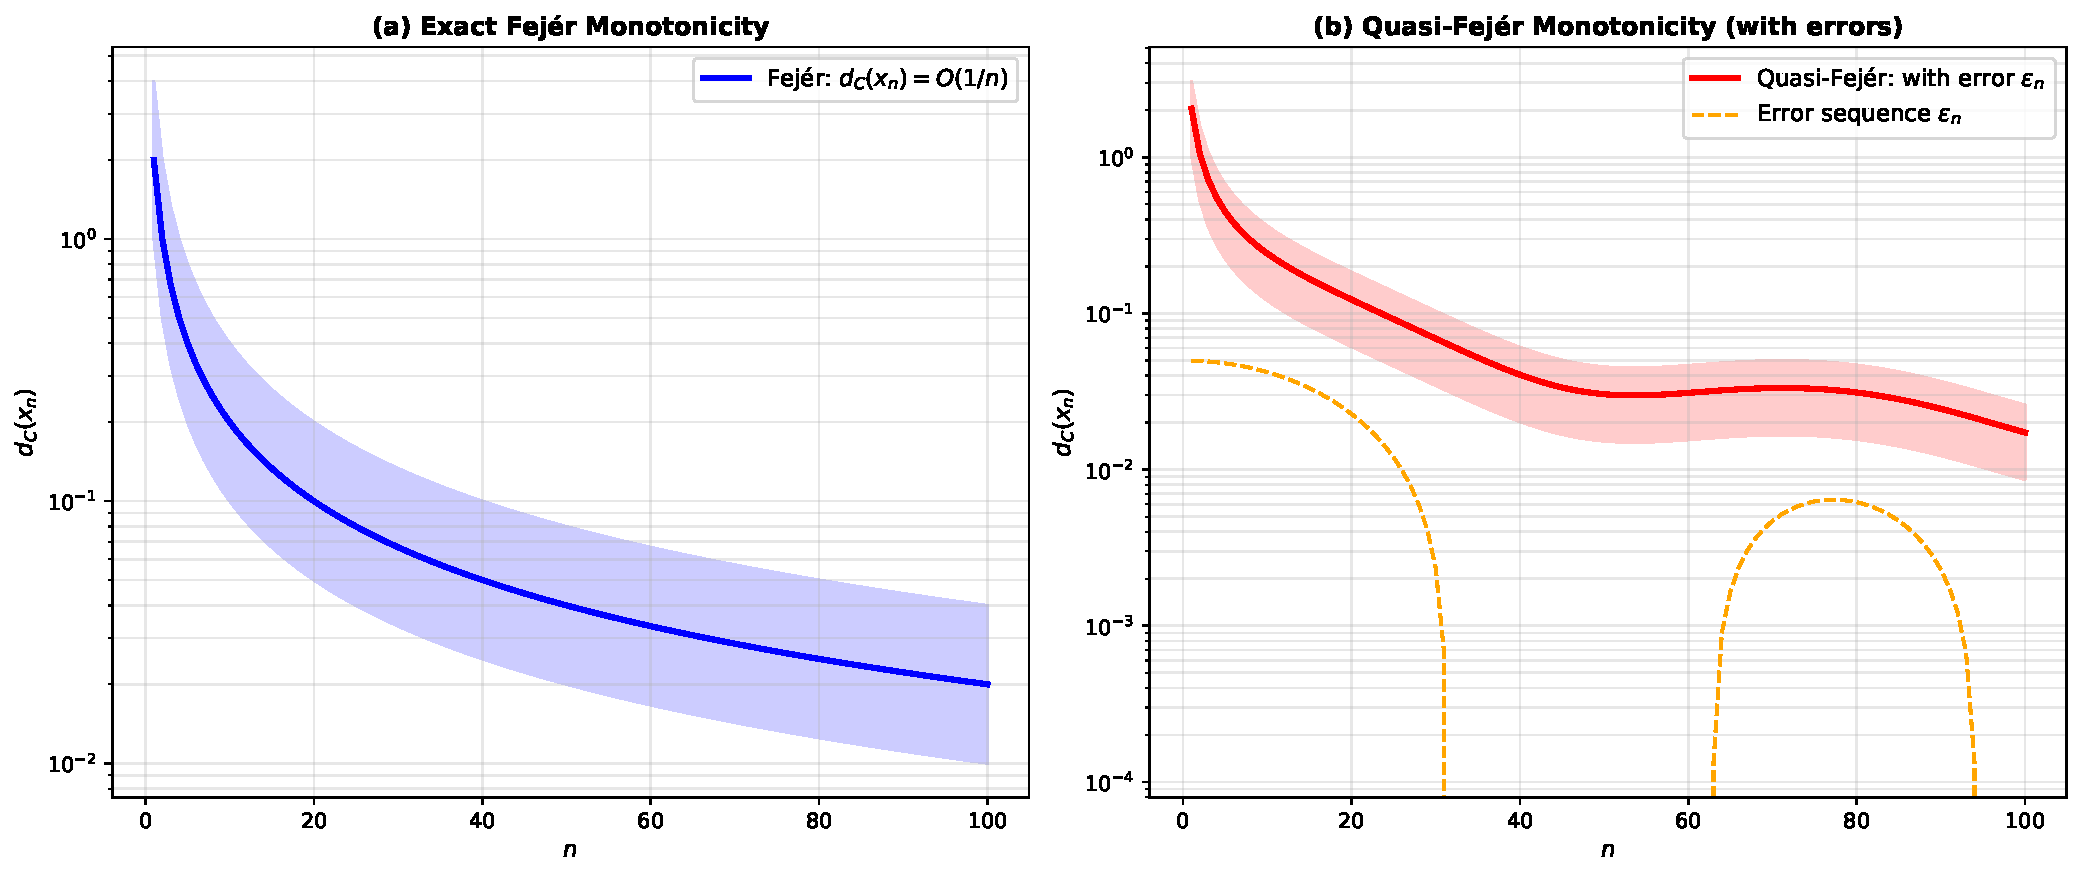
\includegraphics[width=0.72\linewidth]{quasi_fejer.pdf}\\
  {\scriptsize A synthetic quasi-Fej\'er sequence: $\norm{x_{n+1}-x}^2$
  can bump \emph{above} $\norm{x_n-x}^2$ at individual steps (unlike
  strict Fej\'er monotonicity), but only within a summable error
  budget $\varepsilon_n$ -- the dashed envelope from Lemma 5.31 still
  forces overall convergence.}
\end{frame}

\begin{frame}[fragile]{Python: \S5.4 --- Perturbed KM with Summable Error}
  \begin{lstlisting}[style=python]
import numpy as np

def T(x):
    n = np.linalg.norm(x)
    return x / n if n > 1 else x.copy()

def perturbed_km(x0, lam, n_steps, err_power=2.0, err_scale=0.05):
    """x_{n+1} = x_n + lam*(T(x_n) + e_n - x_n),
       e_n = err_scale/(n+1)**err_power * (1,0)  (summable if err_power>1)."""
    x = np.array(x0, dtype=float)
    hist = [x.copy()]
    for n in range(n_steps):
        e_n = np.array([err_scale / (n + 1) ** err_power, 0.0])
        x = x + lam * (T(x) + e_n - x)
        hist.append(x.copy())
    return np.array(hist)

xstar = np.array([0.6, 0.8])
orbit_clean = perturbed_km([3.0, 4.0], 0.5, 10, err_scale=0.0)
orbit_pert  = perturbed_km([3.0, 4.0], 0.5, 10, err_power=2.0, err_scale=0.05)
for n in range(11):
    ec = np.linalg.norm(orbit_clean[n] - xstar)
    ep = np.linalg.norm(orbit_pert[n]  - xstar)
    print(f"n={n:2d}: clean err={ec:.4f}   perturbed err={ep:.4f}")
# Both sequences converge to x* = (0.6, 0.8); the perturbed one tracks
# the clean geometric decay with a small, bounded extra deviation,
# exactly as Proposition 5.34 predicts for summable (lambda_n ||e_n||).
  \end{lstlisting}
\end{frame}

% =================================================================
\section{5.5 Nonlinear Ergodic Theorems}
% =================================================================

\begin{frame}{5.5 Motivation: Averaging a Divergent Sequence}
  Some nonexpansive iterations \textbf{do not converge at all} (e.g.\ a
  rotation: $\Fix T=\{0\}$ but $T^kx_0$ just cycles around a circle
  forever). \textbf{Ergodic theorems} rescue a form of convergence: the
  \textbf{Ces\`aro (running) average} of the iterates converges, even
  when the iterates themselves do not. This section builds the
  abstract principle (Theorem 5.36) and then specializes it to
  Baillon's classical nonlinear ergodic theorem (Example 5.38).
\end{frame}

\begin{frame}[allowframebreaks]{5.5 Theorem 5.36: The Abstract Ergodic Principle}
  \begin{block}{Theorem 5.36}
    Let $(x_n),(y_n)\subset\cH$, $C\ne\emptyset$, and
    $C_m=\overline{\conv}\{y_k\}_{k\ge m}$ for each $m\in\N$. Suppose:
    (i) $(y_n)$ is quasi-Fej\'er monotone w.r.t.\ $C$; (ii)
    $\dC[C_m](x_n)\to0$ for every $m$; (iii) every weak sequential
    cluster point of $(x_n)$ is in $C$. Then $x_n\weakto$ a point in
    $C$.
  \end{block}
  \textbf{Reading it.} $(x_n)$ (typically a Ces\`aro-type average of
  $(y_n)$) need not itself be quasi-Fej\'er --- only \emph{eventually
  close}, in the sense of (ii), to the closed convex hull of the
  \emph{tail} of a quasi-Fej\'er sequence $(y_n)$. This is precisely
  the abstraction needed to justify replacing a divergent orbit by its
  running average.

  \textbf{Proof idea (same polarization trick as Theorem 5.5).} By
  (i) and Theorem 5.33(ii), $(y_n)$ is bounded, hence so is every
  $C_m$, hence so is $(x_n)$ (by (ii)). By (iii) it suffices to rule
  out two distinct weak cluster points $x,z\in C$. Using (i), Theorem
  5.33(i), and the polarization identity
  $$2\inner{y_n}{x-z}=\norm{y_n-z}^2-\norm{y_n-x}^2+\norm x^2-\norm z^2,$$
  $(\inner{y_n}{x-z})_n$ converges to some $\ell\in\R$.

  \framebreak

  \textbf{Squeezing $x_n$ between $y_n$ and its hull.} Fix
  $\varepsilon>0$ and the closed convex set
  $Q=\{y\in\cH:\abs{\inner{y}{x-z}-\ell}\le\varepsilon\}$; for $m$
  large, $(y_n)_{n\ge m}\subset Q$, so $C_m\subset Q$, and (ii) gives,
  for $n$ large,
  $$\norm{x_n-P_Qx_n}=d_Q(x_n)\le d_{C_m}(x_n)\le\varepsilon,\qquad
  \abs{\inner{P_Qx_n}{x-z}-\ell}\le\varepsilon.$$
  Hence $\abs{\inner{x_n}{x-z}-\ell}\le\varepsilon(\norm{x-z}+1)$ for
  $n$ large. Taking limits along subsequences $x_{k_n}\weakto x$ and
  $x_{l_n}\weakto z$ (and $\varepsilon\downarrow0$) gives
  $\inner{x}{x-z}=\ell=\inner{z}{x-z}$, so $\norm{x-z}^2=0$: $x=z$.
  $\blacksquare$
\end{frame}

\begin{frame}{5.5 Corollary 5.37: Weighted Ergodic Averages}
  \begin{block}{Corollary 5.37}
    $(y_n)$ quasi-Fej\'er monotone w.r.t.\ $C$; $(\alpha_{n,k})_{0\le
    k\le n}\subset[0,1]$ with $\sum_{k=0}^n\alpha_{n,k}=1$ for every
    $n$ and $\lim_n\alpha_{n,k}=0$ for every fixed $k$; set
    $$x_n=\textstyle\sum_{k=0}^n\alpha_{n,k}\,y_k. \tag{5.52}$$
    If every weak sequential cluster point of $(x_n)$ lies in $C$,
    then $x_n\weakto$ a point in $C$.
  \end{block}
  \textbf{Symbols:} $\alpha_{n,k}$ = the weight given to the
  \emph{old} iterate $y_k$ when forming the $n$-th running average
  $x_n$; the two conditions say the weights form a genuine convex
  combination at each $n$, and any \emph{fixed} past index $k$'s
  influence vanishes as $n\to\infty$ (so $x_n$ is dominated by
  \emph{recent} $y_k$'s, not stuck on the earliest ones).
  \textbf{Proof idea:} verify Theorem 5.36's hypothesis (ii) directly:
  $d_{C_m}(x_n)\le2\mu\sum_{k=0}^{m-1}\alpha_{n,k}\to0$ as $n\to\infty$
  for fixed $m$, where $\mu=\sup_k\norm{y_k}<\infty$ by Theorem 5.33(ii).
\end{frame}

\begin{frame}[allowframebreaks]{5.5 Example 5.38: Baillon's Nonlinear Ergodic Theorem}
  \begin{block}{Example 5.38 (Baillon)}
    Let $D$ be nonempty closed convex, $T:D\to D$ nonexpansive with
    $\Fix T\ne\emptyset$, $x_0\in D$, and the \textbf{Ces\`aro average
    of Picard iterates}
    $$x_n=\frac{1}{n+1}\sum_{k=0}^nT^kx_0. \tag{5.55}$$
    Then $(x_n)$ converges \textbf{weakly} to a point in $\Fix T$ ---
    \textbf{even if the raw Picard iterates $T^kx_0$ themselves do not
    converge at all.}
  \end{block}

  \textbf{Proof.} Set $C=\Fix T$, $y_k=T^kx_0$. By Example 5.3,
  $(y_k)$ is Fej\'er (hence quasi-Fej\'er) monotone w.r.t.\ $C$. Set
  $\alpha_{n,k}=1/(n+1)$ for $0\le k\le n$: the hypotheses of
  Corollary 5.37 hold ($\sum_k\alpha_{n,k}=1$, $\alpha_{n,k}\to0$ for
  fixed $k$). It remains to show every weak cluster point of $(x_n)$
  is in $C$, and by Cor.\ 4.28 it suffices to show $x_n-Tx_n\to0$.

  \framebreak

  \textbf{Bounding $\norm{Tx_n-z_n}$, where
  $z_n=\tfrac1{n+1}\sum_{k=0}^ny_{k+1}$.} Using the elementary
  telescoping/summation identity for Fej\'er monotone sequences
  (Prop.\ 4.8(iv) and Prop.\ 5.4(iv)),
  $$\norm{Tx_n-z_n}^2\le\frac{1}{2(n+1)^2}\sum_{k=0}^n\sum_{l=0}^n
  \bigl(\norm{y_k-y_l}^2-\norm{y_{k+1}-y_{l+1}}^2\bigr)
  \le\frac{2n\,\dC^2(x_0)}{(n+1)^2}\to0. \tag{5.56}$$

  \textbf{Bounding $\norm{z_n-x_n}$.} A telescoping sum collapses to
  just the first and last terms:
  $$\norm{z_n-x_n}=\frac{1}{n+1}\norm{y_{n+1}-y_0}\le\frac{2\dC(x_0)}{n+1}\to0. \tag{5.57}$$

  \textbf{Conclusion.} $\norm{Tx_n-x_n}\le\norm{Tx_n-z_n}+\norm{z_n-x_n}\to0$,
  so $Tx_n-x_n\to0$; combined with Corollary 5.37 (applicable since
  cluster points now lie in $\Fix T$ via Cor.\ 4.28), $x_n\weakto$ a
  point in $\Fix T$. $\blacksquare$

  \textbf{Why this is remarkable.} No relaxation, no averaging of the
  \emph{operator} was used -- $y_k=T^kx_0$ is the \emph{raw},
  unrelaxed Picard orbit, which can fail to converge entirely (e.g.\ a
  rotation). Averaging \emph{after the fact} (Ces\`aro-summing the
  orbit) is enough to recover weak convergence to a fixed point ---
  a genuinely different mechanism from KM relaxation \emph{during} the
  iteration (\S5.2).
\end{frame}

\begin{frame}{Figure: Baillon's Theorem --- A Rotation Example}
  \centering
  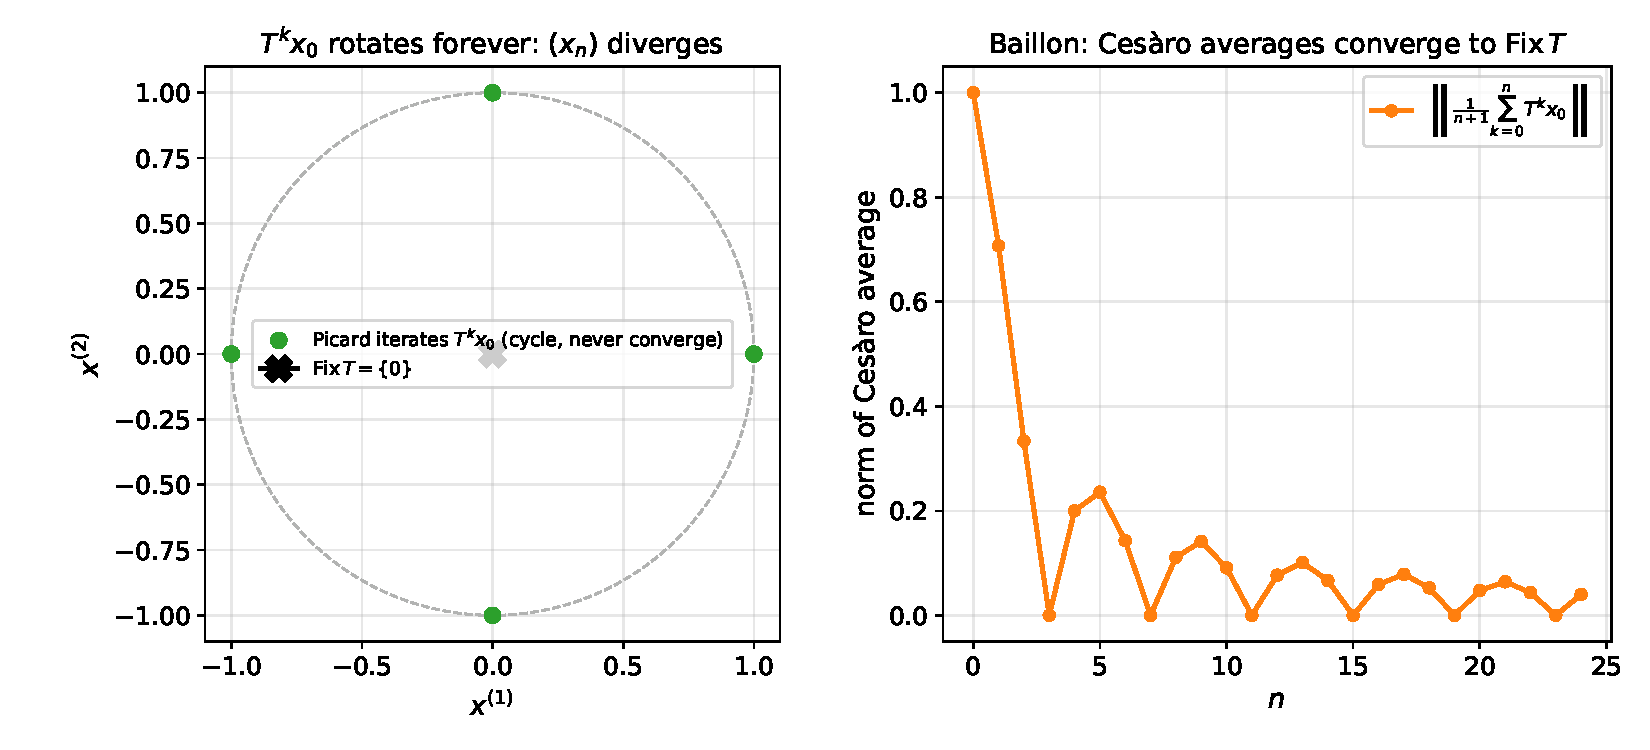
\includegraphics[width=0.92\linewidth]{baillon_ergodic.pdf}\\
  {\scriptsize $T(x,y)=(-y,x)$ (rotation by $90^\circ$): nonexpansive,
  $\Fix T=\{0\}$. \emph{Left:} the raw Picard iterates $T^kx_0$ cycle
  around the unit circle forever and never converge. \emph{Right:} the
  Ces\`aro averages $\frac1{n+1}\sum_{k=0}^nT^kx_0$ nonetheless spiral
  in to $0\in\Fix T$, exactly as Example 5.38 (Baillon) predicts.}
\end{frame}

\begin{frame}[fragile]{Python: \S5.5 --- Baillon's Ergodic Theorem for a Rotation}
  \begin{lstlisting}[style=python]
import numpy as np

def T_rot(x):
    """Rotation by 90 degrees: nonexpansive isometry, Fix(T) = {0}."""
    return np.array([-x[1], x[0]])

x0 = np.array([1.0, 0.0])
N = 12
picard = [x0.copy()]
x = x0.copy()
for _ in range(N):
    x = T_rot(x)
    picard.append(x.copy())
picard = np.array(picard)                       # T^k x0, k=0..N

cesaro = np.cumsum(picard, axis=0) / (np.arange(N + 1).reshape(-1, 1) + 1)

print("Picard norms (never -> 0, just cycles on the unit circle):")
print(np.round(np.linalg.norm(picard, axis=1), 3))
print("Cesaro-average norms (-> 0, i.e. -> Fix(T), by Baillon's theorem):")
print(np.round(np.linalg.norm(cesaro, axis=1), 4))
  \end{lstlisting}
  \textbf{Output pattern.} The Picard norms are all exactly $1$ forever
  (pure rotation on the unit circle); the Ces\`aro-average norms decay
  toward $0$ in an oscillating-but-shrinking pattern, illustrating
  Example 5.38 concretely.
\end{frame}

\begin{frame}{Chapter 5 Summary}
  \begin{itemize}
    \item \textbf{5.1} Fej\'er monotonicity w.r.t.\ $C$ = distances to
      every point of $C$ are non-increasing. Alone, it already forces
      boundedness, convergence of $\norm{x_n-x}$ for all $x\in C$, weak
      convergence once cluster points lie in $C$ (Theorem 5.5), strong
      convergence of the shadow sequence $P_Cx_n$ (Prop.\ 5.7), and
      linear rates under a contraction-type condition on $\dC(x_n)$.
    \item \textbf{5.2} The Krasnosel'ski\u{i}--Mann iteration
      $x_{n+1}=x_n+\lambda_n(Tx_n-x_n)$ with
      $\sum\lambda_n(1-\lambda_n)=\infty$ produces a Fej\'er monotone
      sequence w.r.t.\ $\Fix T$ and drives the residual $Tx_n-x_n\to0$:
      \S5.1's machinery then gives weak convergence for free.
    \item \textbf{5.3} Iterating a fixed \emph{composition} of averaged
      operators is asymptotically regular and weakly convergent along
      cyclically linked subsequences (POCS, von Neumann--Halperin).
    \item \textbf{5.4} Quasi-Fej\'er monotonicity (summable slack
      $\varepsilon_n$) preserves essentially all of \S5.1's
      conclusions --- robust to summable computational error.
    \item \textbf{5.5} Ces\`aro-averaging a (possibly divergent!)
      Fej\'er monotone orbit still converges weakly to the target set
      (Baillon) -- a genuinely different route to convergence.
  \end{itemize}
\end{frame}

\end{document}
